\section{Verification}
\label{app:verification}

%\subsection{Polynomial Reproducibility}

One of the most important tests is to numerically confirm the polynomial approximability properties of the spaces spanned by the shape functions.
Coupled with the exact sequence property of the discrete spaces, this ensures all well known interpolation inequalities.
More specifically, for an affinely transformed master element mesh, let $W^p$ be the span of the $H^1$ basis functions of order $p$ (being composed piecewise by shape functions), and similarly with $Q^p$, $V^p$ and $Y^p$ for the spaces $H(\mathrm{curl})$, $H(\mathrm{div})$ and $L^2$ respectively.
Then, one has to check that $\mathcal{P}^p\subseteq W^p$, $(\mathcal{P}^{p-1})^3\subseteq Q^p$, $(\mathcal{P}^{p-1})^3\subseteq V^p$ and $\mathcal{P}^{p-1}\subseteq Y^p$.

To do this, first consider an arbitrary $u$ in a given energy space $U$ approximated by a discrete space $U_h$.
Clearly,
\begin{equation}
	u\in U_h \Leftrightarrow \mathrm{dist}(u,U_h)=\min_{u_h\in U_h}||u-u_h||_U=0\,.
\end{equation}
Hence, given $u\in U$ the task is to compute $\mathrm{dist}(u,U_h)=||u-u_h||_U$, with $u_h\in U_h$ being the element where the minimum is attained.
Fortunately $u_h$ is computed from a variational problem equivalent to the projection (distance) problem.
It is,
\begin{equation}
	||u-u_h||_U=\mathrm{dist}(u,U_h)\Leftrightarrow
		\begin{cases}
			u_h\in U_h\,,&{}\\
			b(u_h,v_h)=\langle u_h,v_h \rangle_U=\langle u,v_h \rangle_U=\ell_u(v_h)& \forall v_h\in U_h.
		\end{cases}
	\label{eq:variationalprojection}
\end{equation}
Naturally, the inner product is different depending on the energy space $U$.
They are,
\begin{equation}
  \begin{aligned}
	  \langle \phi_1,\phi_2\rangle_{H^1}&=\int_\Omega (\phi_1\phi_2+\nabla\phi_1\cdot\nabla\phi_2)\mathrm{d}\Omega\,,\\
	  \langle E_1,E_2\rangle_{H(\mathrm{curl})}&=\int_\Omega (E_1\cdot E_2+(\nabla\times E_1)\cdot(\nabla\times E_2))\mathrm{d}\Omega\,,\\
		\langle V_1,V_2\rangle_{H(\mathrm{div})}&=\int_\Omega (V_1\cdot V_2+(\nabla\cdot V_1)(\nabla\cdot V_2))\mathrm{d}\Omega\,,\\
		\langle \psi_1,\psi_2\rangle_{L^2}&=\int_\Omega \psi_1\psi_2\mathrm{d}\Omega\,.
	\end{aligned}
\end{equation}

Then, the task is to determine whether each element $u$ of a monomial basis for the polynomial spaces in question lies in $U_h$.
This is achieved by solving the variational problem in \eqref{eq:variationalprojection} and checking that the relative error $\frac{||u-u_h||_U}{||u||_U}=\frac{\mathrm{dist}(u,U_h)}{||u||_U}$ is in the range of machine zero.
Thus, for example to ensure that $\mathcal{P}^p\subseteq W^p$ one must check that all monomials of the form $x^iy^jz^k$ for $i+j+k\leq p$ lie in $W^p$, the span of the $H^1$ basis functions.
Similar procedures hold for $H(\mathrm{curl})$, $H(\mathrm{div})$ and $L^2$.
These tests are called \textit{polynomial reproducibility} tests.

The polynomial reproducibility tests are successful when using the code associated with this work.
The tests are done on a series of meshes, including a four element hybrid mesh with one element of each type, as depicted in Figure \ref{fig:VerificationMesh}.
By doing this on a mesh, there is the additional value of implicitly verifying compatibility of the shape functions across the boundaries of the elements.
Indeed, it should be checked that the polynomial reproducibililty tests pass under all possible orientations of each face and edge in the mesh, which is the case for our code.

\begin{figure}[!ht]
\begin{center}
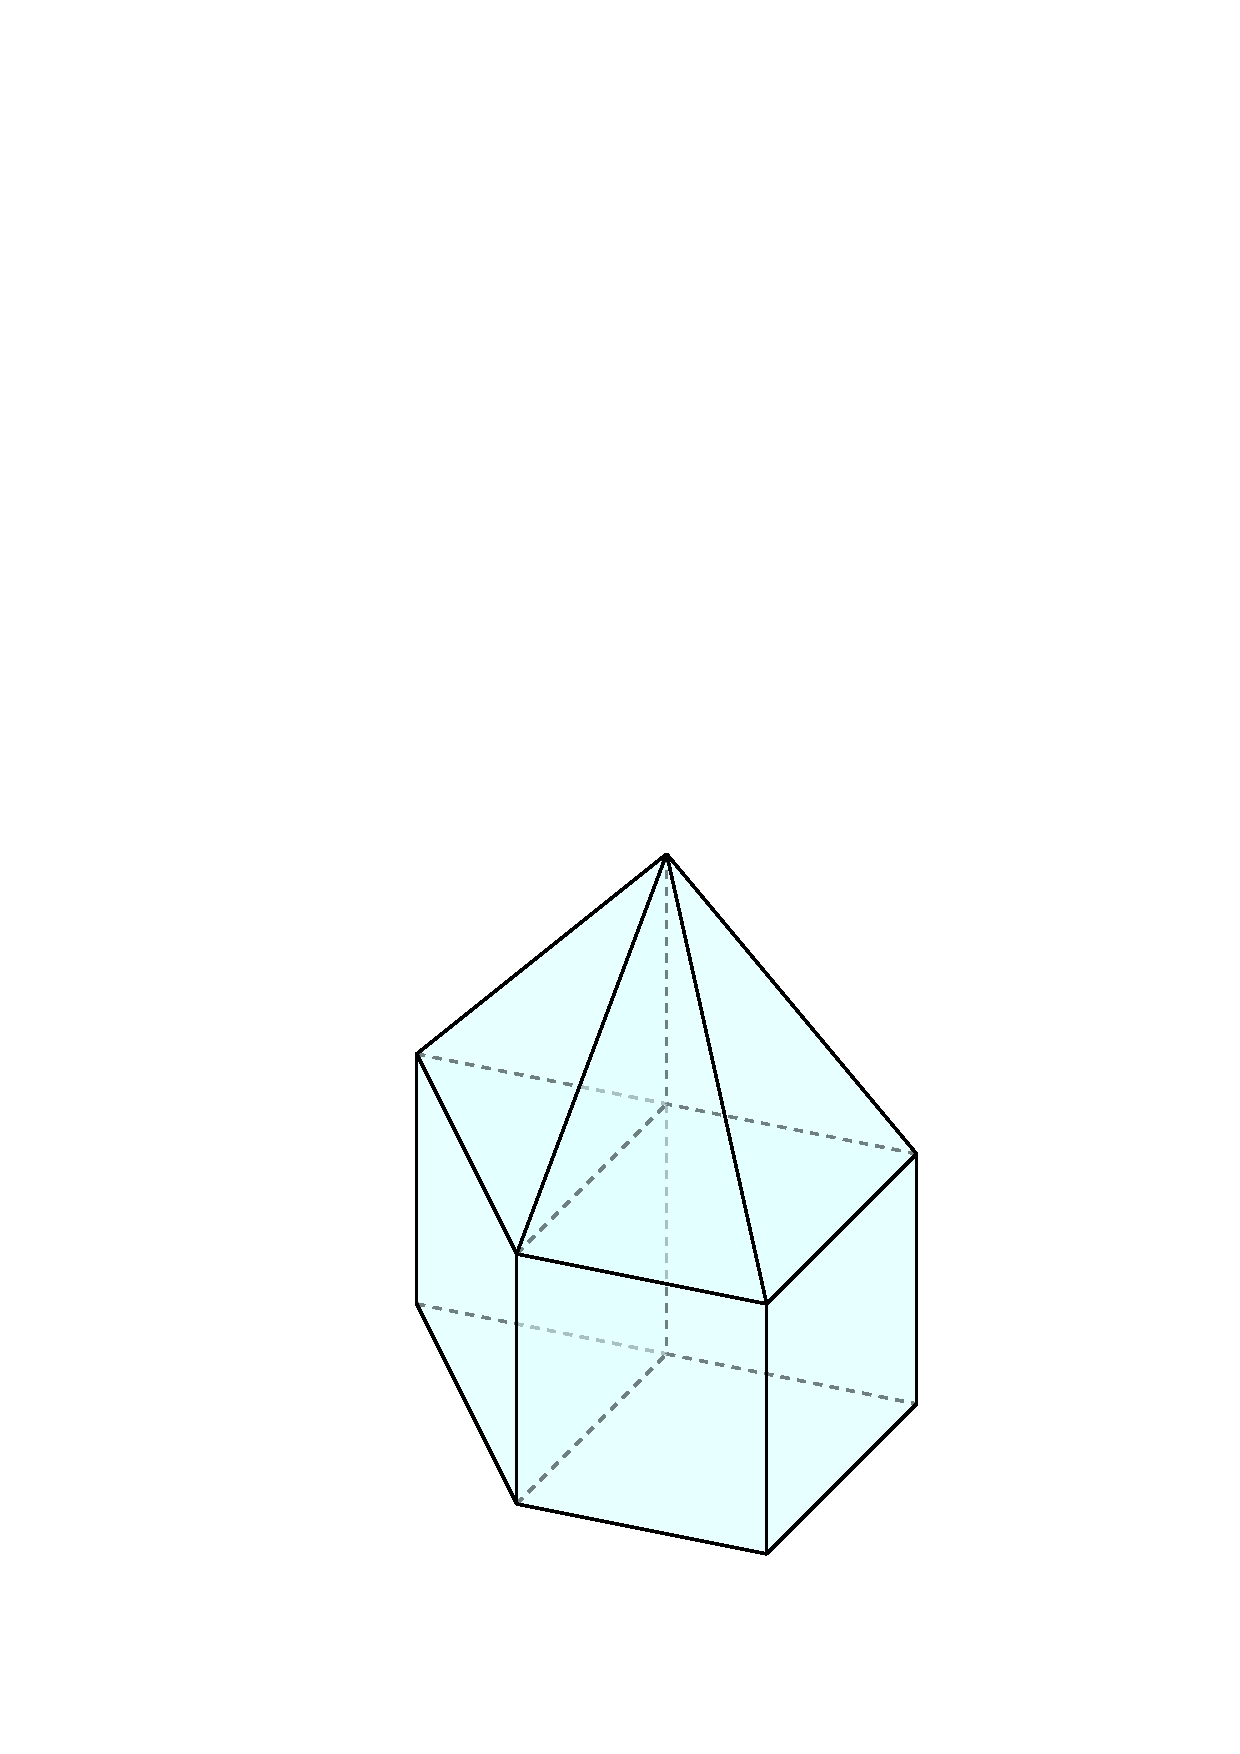
\includegraphics[scale=0.5]{./figures/VerificationMesh.pdf}
\caption{A hybrid mesh used to verify polynomial reproducibility.}
\label{fig:VerificationMesh}
\end{center}
\end{figure}

%\subsection{Exact Sequence Properties}

Another convenient test is to verify some aspects of the exact sequence property of the discrete spaces.
For this, consider a fixed element and the discrete spaces $W^p$, $Q^p$, $V^p$ and $Y^p$ conforming to $H^1$, $H(\mathrm{curl})$, $H(\mathrm{div})$ and $L^2$ respectively.
The discrete spaces are precisely the span of the corresponding shape functions.

Hence, for example consider an $H^1$ shape function $\phi\in W^p$.
Then the idea is to confirm numerically that $\nabla\phi\in Q^p$.
This is done as described in the polynomial reproducibility tests, where the computed projection of $\nabla\phi$ to $Q^p$ is $E_h$, which is given as a linear combination of the $H(\mathrm{curl})$ shape functions $E\in Q^p$.
Therefore, one should obtain that that $\frac{||\nabla\phi-E_h||_{H(\mathrm{curl})}}{||\nabla\phi||_{H(\mathrm{curl})}}$ is in the range of machine zero.
Moreover, one can additionally check that the coefficients of the linear combination for $E_h$ make sense.
For instance, if $\phi\in W^p$ is originally an $H^1$ interior bubble, then $\nabla\phi$ is also an $H(\mathrm{curl})$ interior bubble and as a result is in the span of the $H(\mathrm{curl})$ interior shape functions (meaning the coefficients associated to $H(\mathrm{curl})$ edge and face shape functions are zero).
Similarly, if $\phi\in W^p$ is an $H^1$ face shape function, then $\nabla\phi$ is in the span of the the $H(\mathrm{curl})$ face functions associated to the same face \textit{and} the $H(\mathrm{curl})$ interior bubbles.
Naturally this applies to other topological entities and to the different energy spaces.

These verifications are successful when using the code that supplements this text.


%\begin{equation}
%\begin{aligned}
%	u\in U_h&\Leftrightarrow \mathrm{dist}(u,U_h)=\min_{u_h\in U_h}||u-u_h||_U=0\\&\Leftrightarrow
%		\begin{cases}
%			u_h\in U_h\,,&{}\\
%			b(u_h,v_h)=\langle u_h,v_h \rangle_U=\langle u,v_h \rangle_U=\ell_u(v_h)& \forall v_h\in U_h.
%		\end{cases}
%\end{aligned}
%\end{equation}
%This is called the projection problem to $U_h$ from $U$

%
%\subsection{Reproducing Polynomials.}
%
%Consider the $H^1$-projection problem:
%$$
%\int_{\Omega} [(\bfnab u_h - \bfnab u) \bfnab v_h + (u_h - u) v_h] = 0
%\quad \forall v_h \, .
%$$
%If projected function $u$ lives in the FE space, the FE solution $u_h$ must coincide
%with $u$ up to machine precision, and the corresponding relative $H^1$ error is expected
%to be of order $10^{-15}$. Given the four element mesh shown in
%Fig.~\ref{fig:verification} with order\footnote{More precisely, the tet and pyramid
%are of order $p$, hexa is of order $ppp$, and prism is of order $pp$.} of elements set to $p$,
% we loop through monomials
%$$
%u = x^i y^j z^k,\quad i,j,k \geq 0,\,  i+j+k \leq p\, ,
%$$
%and verify that, for each projected monomial, the projection error is indeed in the range of machine zero.
%
%We perform the same test for $H(\text{curl})$-conforming elements and $H(\text{curl})$ projection,
%$$
%\int_{\Omega} [(\bfnab \times E_h - \bfnab \times E) \cdot \bfnab \times F_h + (E_h - E) \cdot F_h] = 0
%\quad \forall F_h \, ,
%$$
%using several familes of vector polynomials $E$,
%$$
%\begin{array}{ll}
%E = x^i y^j z^k e \quad & i,j,k \geq 0,\,  i+j+k \leq p-1\, ,\\
%E = x^i y^j z^k (x,y,z) \times \bfe & i,j,k \geq 0,\,  i+j+k = p-1\,
%\end{array}
%$$
%where $e = (1,0,0), \, (0,1,0), \, (0,0,1)$.
%
%
%Similarly, for $H(\text{div})$-conforming elements we use the $H(\text{div})$ projection,
%$$
%\int_{\Omega} [(\bfnab \cdot V_h - \bfnab \cdot V) \bfnab \cdot W_h + (V_h - V) \cdot W_h] = 0
%\quad \forall W_h \, ,
%$$
%using the following familes of vector polynomials $V$,
%$$
%\begin{array}{ll}
%F = x^i y^j z^k e \quad & i,j,k \geq 0,\,  i+j+k \leq p-1\, ,\\
%F = x^i y^j z^k (x,y,z)  & i,j,k \geq 0,\,  i+j+k = p-1\, .
%\end{array}
%$$
%Finally, we use the $L^2$-projection and monomials of order $p-1$ to verify the $L^2$-conforming
%elements.
%
%
%
%
%
%
%\begin{figure}[ht!]
%\begin{center}
%\includegraphics[angle=0,width=0.50\textwidth]{./figures/verification.png}
%\end{center}
%\caption{Four element mesh used for the verification.
%}
%\label{fig:verification}
%\end{figure}
%
%
%\subsection{Verifying Orientations.} In the next test, for every edge and every face
%in the mesh, we loop through all possible edge and face orientations (two for edge, six for a triangle,
%and eight for a square) and, for each modified orientation, perform the projection test
%described above. All edges and faces are explicitly defined in a geometry input file
%by listing the corresponding edge-to-vertex and face-to-vertex connectivities. Changing
%the orientations reduces thus to listing the vertices in a different order. For instance,
%the vertices for square face $1265$ undergo the following permutations:
%$$
%1265,\quad 2651,\quad 6512,\quad 5126,\quad 1562,\quad 2156,\quad 6215,\quad 5621 \, .
%$$
%
%\subsection{Verifying Exact Polynomial Complex Property}
%
%One of the tools that we have found very useful
%was the verification of the polynomial complex property. For instance, the $H(\text{curl})$ elements
%(one element at a time) we debugged by using $E = \bfnab u_h$ where $u_h$ is an $H^1$ shape function.
%Not only we know that the correponding projection error must be zero but also we know ahead of time
%which $H(\text{curl})$ shape functions should contribute to (``connect with'') the projection.
%For instance, if $u_h$ is an element $H^1$ bubble then $E_h$ must also be an element  $H(\text{curl})$
%bubble. Similarly, if $u_h$ is a face bubble then $E_h$ must live in the span of the same face
%$H(\text{curl})$ bubbles and element bubbles, etc. This verification helped to eliminate not only
%coding errors but also a few theoretical omittments (for the pyramid) as well.
%
%\subsection{Other Useful Debugging Tools}
%
%When encountering an error in performing the projection tests for the $H(\text{curl})$
%and $H(\text{div})$, we frequently switched to $L^2$ projections. This helps to separate debugging
%the formulas for the $H(\text{curl})$
%and $H(\text{div})$ shape functions from the corresponding formulas for their curl and divergence.
